\chapter{Performance MIDI-to-Score Conversion by Neural Beat Tracking}

The main model of interest \cite{Liu2022} is composed of two parts:
\begin{itemize}
	\item Beat Tracking.
	\item Score Element Assignment.
\end{itemize}

The first part is responsible for quantizing the raw material into beats and downbeats. Each measure is consisted of several beats, and the number of beats in a measure is governed by the time signature. The beats mark the tempo, and they are the basis for the musical onsets detection.

The second part assigns every other aspect of the musical score to the MIDI stream. Let us recall these elements: musical onsets, note values, hand parts, key signature and time signature.

Let us review both components.

\section{Beat Tracking}

A single measure consists of several beats, and the rhythmic structure of beats is determined by time signature (or signatures). A performance MIDI does not contain information about beats and one of the objectives of the model is to predict locations of these.

After these predictions, note beginnings (onsets) can be placed in a subdivision of a single beat. The smallest unit of time distance is thus dictated by the size of the beat subdivision. More precisely, a musical onset $mo_i$ of the $i$-th note is defined as \[mo_i = \frac{s_n}{S}\] where $S$ is the number of subdivisions per beat in rhythm quantization, and $s_n$ is the musical onset time expressed in the number of subdivisions.

The authors provide a novel approach to detecting beats, splitting them into two categories, for which there are two separate methods.

Beats can fall into two distinct groups:
\begin{itemize}
	\item \emph{In-note}: beats concurrent with at least one note onset. This means that some notes play within the start of the beat.
	\item \emph{Out-of-note}: a beat is not concurrent with any note onset. No notes are beginning with such beats.
\end{itemize}

\subsection{In-note Beat Prediction}

For predicting in-note beats, one can reduce the problem to a binary classification task on the note sequence $\mathbf{X}$. This sequence is assumed to have a length $N$.

\begin{figure}[!ht]
\centering
\begin{tikzpicture}
\tikzset{layer1/.style={fill=gray!10, draw=gray, thick, text centered}}
\tikzset{layer2/.style={fill=gray!30, draw=gray, thick, text centered}}
\tikzset{arrowstyle/.style={-{Latex[length=3mm]}}}

	\fill[fill=gray!50, fill opacity=0.5, draw=gray, thick, line width=2pt] (0.0, 0.0) rectangle (12.0, 7.0);
	\fill[fill=gray!30, fill opacity=0.5, draw=gray, thick, line width=2pt] (0.0, -0.5) rectangle (12.0, -4.0);
	\fill[fill=white!50, fill opacity=1.0, draw=black, thick, line width=1pt] (0.5, 2.0) rectangle (10.5, 6.5);
	\fill[fill=white!50, fill opacity=1.0, draw=black, thick, line width=1pt] (1.0, 1.5) rectangle (11.0, 6.0);
	\fill[fill=white!50, fill opacity=1.0, draw=black, thick, line width=1pt] (1.5, 1.0) rectangle (11.5, 5.5);

    \draw (6.5, 7.75) node (note_sequence) {Note sequence};
    \draw (6.5, 4.75) node[layer2] (layerA1) {Convolutional};
    \draw (6.5, 3.75) node[layer1] (layerA2) {Batch normalization};
    \draw (6.5, 2.75) node[layer1] (layerA3) {Exponential linear unit};
    \draw (6.5, 1.75) node[layer1] (layerA4) {Dropout};
    \draw[anchor=south, inner sep=2pt] (6.5, 0.0) node (outputA) {To the next convolutional layer};
    
    \draw (6.5, -1.25) node[layer2] (layerB1) {Bi-directional GRU (512)};
    \draw (6.5, -2.25) node[layer2] (layerB2) {Bi-directional GRU (512)};
    \draw (6.5, -3.25) node[layer1] (layerB3) {Linear (512)};
    
    \draw (6.5, -5.00) node[layer1] (output) {Linear (1)};
    
	\node[anchor=south west, inner sep=2pt] at (0.2, 0.2) {ConvBlock};    
	\node[anchor=south west, inner sep=2pt] at (0.2, -3.8) {GRUBlock};
	
	\node[anchor=north west, inner sep=2pt] at (1.55, 5.45) {\small{(9, in features), 128}};
	\node[anchor=north west, inner sep=2pt] at (1.05, 5.95) {\small{(9, 1), 256}};
	\node[anchor=north west, inner sep=2pt] at (0.55, 6.45) {\small{(9, 1), 512}};
	\node[anchor=north west, inner sep=2pt] at (0.05, 6.95) {\small{kernel size, channels}};
	
	\draw[arrowstyle] (note_sequence.south) to (layerA1.north);
	\draw[arrowstyle] (layerA1.south) to (layerA2.north);
	\draw[arrowstyle] (layerA2.south) to (layerA3.north);
	\draw[arrowstyle] (layerA3.south) to (layerA4.north);
	\draw[arrowstyle] (layerA4.south) to (outputA.north);
	\draw[arrowstyle] (layerA4.south) to (outputA.north);
	
	\draw[arrowstyle] (outputA.south) to (layerB1.north);
	\draw[arrowstyle] (layerB1.south) to (layerB2.north);
	\draw[arrowstyle] (layerB2.south) to (layerB3.north);
	\draw[arrowstyle] (layerB3.south) to (output.north);
\end{tikzpicture}
\caption[In-note beat prediction model]{In-note beat prediction model with a CRNN with 3 convolutional layers and 2 bi-directional gated recurrent unit (GRU) layers.}
\end{figure}

The probability $P_n$ that $n$-th note is concurrent with a beat is defined as: \[P_n = \mathbb{P}\left(B_n|\mathbf{X}\right)\] where $B_n\in\{0,1\}$ is the ground-truth beat label for the $n$-th note from the note sequence. The model is trained using the standard cross-entropy loss function: \[\mathcal{L}=-\frac{1}{N}\sum_{n=1}^N B_n\ln P_n + \left(1-B_n\right)\ln\left(1-P_n\right)\] The authors used CRNN with 3 convolutional layers and 2 bidirectional gated recurrent unit (GRU) layers. The probability threshold for positive classification has been set dynamically, depending on the maximum probability in a fixed segment length.

\subsection{Out-of-note Beat Prediction}

The approach to predicting out-of-note beats, which do not align with note onsets, requires distinct approach. Liu et al. (2022) proposed a dynamic programming strategy to solve this problem \cite{Liu2022}.

Let us assume that there are $B^i$ in-note beats $\{b_n^i\}_{n=1}^{B^i}$ in total, and out-of-note beats are at subdivisions of the neighboring in-note beats\footnote{We may select only one note per in-note beat, if there are more.} $b_{n}^i$ and $b_{n+1}^i$.

The goal of the procedure is to find out-of-note beats $b^o$ from a set of candidates: \begin{equation}\label{out_of_note_candidates}
b_{n,K}^o = \left\{b_n^i + \frac{k}{K+1}\left(b_{n+1}^i-b_n^i\right)\right\}_{k=1}^K
\end{equation} where $K\in\{0,1,2,3\}$ is the number of out-of-note beats to insert inside the $\left(b_{n+1}^i, b_n^i\right)$ interval.

The number of candidates is selected in order to minimize the tempo change after adding out-of-note beats. The function may be represented as the sum: \[\mathcal{O}_1 = \sum_{n=1}^{B-2}\left|\ln\left(\frac{b_{n+2} - b_{n+1}}{b_{n+1} - b_n}\right)\right|\] where $\{b_n\}_{n=1}^B$ is the sequence of all $B$ beats (both in-note and out-of-note, sorted chronologically).

To discourage the procedure from adding too many out-of-note beats, which leads to an unnecessarily subdivided output, an additional penalty is associated with the objective function: \begin{equation}\label{out_of_note_objective}
\mathcal{O} = \mathcal{O}_1 + \lambda B^o
\end{equation} where $B^o$ is the number of added out-of-note beats, and $\lambda$ is the penalty coefficient. The coefficient is to be found experimentally, however the default value set by the authors is $1$.

\begin{algorithm}[ht!]
\begin{algorithmic}[1]
\Require{list of in-note notes $\mathcal{B}^i$}
\Ensure{list of all beats $\mathcal{B}$ including added out-of-note beats}
\State $n \gets 1$
\For{$K=0,1,2,3$}
    \State initialize objective function $\mathcal{O}_K\gets 0$
    \State initialize beat sequence $\mathcal{B}_K\gets \{b_1\}$
\EndFor
\For{$n=1,2,\ldots,B^i-2$}
    \For{$K_{\textrm{cur}}=0,1,2,3$}
        \State get out-of-note beats for current step by \eqref{out_of_note_candidates}
        \If{tempo is beyond tempo range limits}
            \State \textbf{continue}
        \EndIf
        \For{$K_{\textrm{prev}}=0,1,2,3$}
            \State update objective function by \eqref{out_of_note_objective}
        \EndFor
        \State select the minimum objective among all $K_{\textrm{prev}}$ values
        \State add out-of-beats for the current step to the beat sequence mapped to the selected $K_{\textrm{prev}}$
    \EndFor
    \For{$K_{\textrm{cur}}=0,1,2,3$}
        \State update $\mathcal{O}_K$, $\mathcal{B}_K$ mapped with $K_{\textrm{cur}}$
    \EndFor
\EndFor
\State \Return{the beat sequence $\mathcal{B}_K$ with the minimum objective function $\mathcal{O}_K$}
\end{algorithmic}
\captionof{algorithm}[Out-of-note beat prediction.]{Out-of-note beat prediction.}
\end{algorithm}


\section{Score Elements Assignment}

As discussed in the Section \ref{music_score_encoding}, score elements assignment may be viewed as a function from a note sequence $\mathbf{X}$ into a score encoded by a tensor $\mathbf{Y}_n$ representing musical onsets, note values, key signature, time signature, and hand parts, for each note separately.

Besides the quantization model, which relies on the beat tracking module, key signature, time signature and hand parts modules can be treated independently.

\begin{figure}[!ht]
\centering
\begin{tikzpicture}
    \tikzset{sequence/.style={thick, text centered, align=center}}
    \tikzset{convblock/.style={fill=gray!20, draw=gray, thick, text centered}}
    \tikzset{grublock/.style={fill=gray!30, draw=gray, thick, text centered}}
    \tikzset{linear/.style={fill=gray!10, draw=gray, thick, text centered}}
    \tikzset{output/.style={thick, anchor=west, align=left}}
    \tikzset{arrowstyle/.style={-{Latex[length=3mm]}}}
    \draw (-3.5, 0.5) node[sequence] (sequence) {note\\ sequence};

    \draw (-1.75, 5) node (joint1) {};
    \draw (-1.75, 3) node (joint2) {};
    \draw (-1.75, 2) node (joint3) {};
    \draw (-1.75, 0.5) node (joint4) {};
    \draw (-1.75, -1) node (joint5) {};
    \draw (-1.75, -2) node (joint6) {};

    \draw (1.5, 3) node (concatenation) {$\boldsymbol{\oplus}$};
    \draw (1.5, 3.5) node (concatleftjoint1) {};
    \draw (1.5, 2.5) node (concatleftjoint2) {};
    \draw (7.25, 3.5) node (concatrightjoint1) {};
    \draw (7.25, 2.5) node (concatrightjoint2) {};
    \draw (7.25, 2) node (concatstart1) {};
    \draw (7.25, 4) node (concatstart2) {};

    \draw (0, 5) node[convblock] (convblock1) {ConvBlock};
    \draw (0, 3) node[convblock] (convblock2) {ConvBlock};
    \draw (0, 2) node[convblock] (convblock3) {ConvBlock};
    \draw (0, 0.5) node[convblock] (convblock4) {ConvBlock};
    \draw (0, -1) node[convblock] (convblock5) {ConvBlock};
    \draw (0, -2) node[convblock] (convblock6) {ConvBlock};

    \draw (3, 6) node[grublock] (grublock1) {GRUBlock};
    \draw (3, 5) node[grublock] (grublock2) {GRUBlock};
    \draw (3, 4) node[grublock] (grublock3) {GRUBlock};
    \draw (3, 3) node[grublock] (grublock4) {GRUBlock};
    \draw (3, 2) node[grublock] (grublock5) {GRUBlock};
    \draw (3, 0.5) node[grublock] (grublock6) {GRUBlock};
    \draw (3, -1) node[grublock] (grublock7) {GRUBlock};
    \draw (3, -2) node[grublock] (grublock8) {GRUBlock};

    \draw (6, 6) node[linear] (linear1) {Linear (200)};
    \draw (6, 5) node[linear] (linear2) {Linear (1)};
    \draw (6, 4) node[linear] (linear3) {Linear (1)};
    \draw (6, 3) node[linear] (linear4) {Linear (24)};
    \draw (6, 2) node[linear] (linear5) {Linear (96)};
    \draw (6, 1) node[linear] (linear6) {Linear (5)};
    \draw (6, 0) node[linear] (linear7) {Linear (4)};
    \draw (6, -1) node[linear] (linear8) {Linear (12)};
    \draw (6, -2) node[linear] (linear9) {Linear (1)};

    \draw (7.75, 6) node[output] (output1) {tempo};
    \draw (7.75, 5) node[output] (output2) {downbeats};
    \draw (7.75, 4) node[output] (output3) {beats};
    \draw (7.75, 3) node[output] (output4) {musical onsets};
    \draw (7.75, 2) node[output] (output5) {note values};
    \draw (7.75, 1) node[output] (output6) {time signature\\  numerators};
    \draw (7.75, 0) node[output] (output7) {time signature\\  denominators};
    \draw (7.75, -1) node[output] (output8) {key signature};
    \draw (7.75, -2) node[output] (output9) {hand parts};

    \draw (sequence) to (joint4.center);
    \draw (joint1.center) to (joint6.center);
    \draw[arrowstyle] (joint1.center) to (convblock1);
    \draw[arrowstyle] (joint2.center) to (convblock2);
    \draw[arrowstyle] (joint3.center) to (convblock3);
    \draw[arrowstyle] (joint4.center) to (convblock4);
    \draw[arrowstyle] (joint5.center) to (convblock5);
    \draw[arrowstyle] (joint6.center) to (convblock6);

    \draw[arrowstyle] (convblock1.east) to (grublock1.west);
    \draw[arrowstyle] (convblock1.east) to (grublock2.west);
    \draw[arrowstyle] (convblock1.east) to (grublock3.west);
    \draw[arrowstyle] (convblock2.east) to (grublock4.west);
    \draw[arrowstyle] (convblock3.east) to (grublock5.west);
    \draw[arrowstyle] (convblock4.east) to (grublock6.west);
    \draw[arrowstyle] (convblock5.east) to (grublock7.west);
    \draw[arrowstyle] (convblock6.east) to (grublock8.west);

    \draw[arrowstyle] (grublock1.east) to (linear1.west);
    \draw[arrowstyle] (grublock2.east) to (linear2.west);
    \draw[arrowstyle] (grublock3.east) to (linear3.west);
    \draw[arrowstyle] (grublock4.east) to (linear4.west);
    \draw[arrowstyle] (grublock5.east) to (linear5.west);
    \draw[arrowstyle] (grublock6.east) to (linear6.west);
    \draw[arrowstyle] (grublock6.east) to (linear7.west);
    \draw[arrowstyle] (grublock7.east) to (linear8.west);
    \draw[arrowstyle] (grublock8.east) to (linear9.west);

    \draw[arrowstyle] (linear1.east) to (output1.west);
    \draw[arrowstyle] (linear2.east) to (output2.west);
    \draw[arrowstyle] (linear3.east) to (output3.west);
    \draw[arrowstyle] (linear4.east) to (output4.west);
    \draw[arrowstyle] (linear5.east) to (output5.west);
    \draw[arrowstyle] (linear6.east) to (output6.west);
    \draw[arrowstyle] (linear7.east) to (output7.west);
    \draw[arrowstyle] (linear8.east) to (output8.west);
    \draw[arrowstyle] (linear9.east) to (output9.west);

    \draw[arrowstyle, dashed] (concatleftjoint1.center) to (concatenation.center);
    \draw[arrowstyle] (concatleftjoint2.center) to (concatenation.center);
    \draw[dashed] (concatleftjoint1.center) to (concatrightjoint1.center);
    \draw (concatleftjoint2.center) to (concatrightjoint2.center);
    \draw (concatstart1.center) to (concatrightjoint2.center);
    \draw[dashed] (concatstart2.center) to (concatrightjoint1.center);

    \draw (3.5, -3) node[output] (legendsymbol1) {$\boldsymbol{\oplus}$};
    \draw (3, -3.75) node[output] (legendsymbolstart) {};
    \draw (4.5, -3.75) node[output] (legendsymbolend) {};
    \draw (5, -3) node[output] (legend1) {concatenation};
    \draw (5, -3.75) node[output] (legend2) {disable backpropagation during training};
    \draw[arrowstyle, dashed] (legendsymbolstart.center) to (legendsymbolend.center);
\end{tikzpicture}

\caption[The architecture of the model.]{The architecture of the model. There are five separate modules of the entire model in total: \emph{beat}, \emph{quantization}, \emph{time signature}, \emph{key signature} and \emph{hand parts}.}
\end{figure}

\section{Score Generation}

The final score generation process synthesizes the source MIDI stream, incorporating pitch sequence, with the model's output. The resultant annotated MIDI encompasses essential information for visual score generation, including key/time signatures, which are not typically present in standard MIDI files.

\section{Model Performance}

\section{Robustness Analysis}

\subsection{Ceteris Paribus}

We conducted a \emph{ceteris paribus} analysis focusing on musical element models, making several assumptions:

\begin{itemize}[noitemsep, topsep=4pt]
	\item Note velocity should not affect time signature or hand part assignment.
	\item Note duration should not impact key signature.
	\item Note pitch is crucial for key signature/hand part assigning, while other features should not contribute.
	\item Note pitch does not matter for the time signature.
\end{itemize}

These should be regarded as general guidelines rather than strict principles.

\subsubsection{Perturbations}

For a sample $M=50$ musical pieces from the dataset, we introduced perturbations to test the assumptions:

\begin{itemize}[noitemsep, topsep=4pt]
	\item Changing velocity with standard deviations $\sigma_v$ of 8, 16, 32, and 64.
	\item Scaling note lengths by a factor from an interval $\alpha\in(\alpha_l,1)$, where $\alpha_l\in\{0.9, 0.75, 0.5, 0.2\}$ (note extension may lead to overlapping).
	\item Changing pitch with standard deviations $\sigma_p$ of 12 and 24 (whole octave, double octave).
\end{itemize}

Each transformation is applied separately to each feature, note by note. Notice that we don't change onsets as they change the musical structure of a piece.

For each feature model $f$: \emph{hand part} $f_H$, \emph{key signature} $f_K$, \emph{time signature} $f_T$, we calculated the average error between the output sequence and the output of a perturbed sequence.

For each element ${\bf x}_i$ in the dataset sample $i\in\{1,2,\ldots,50\}$ and for each change, we sampled $m=10$ perturbations ${\bf x}^{(j)}$ of the original item and measured the error: \[\operatorname{error}\left(f\right) = \frac{1}{M}\sum_{i=1}^{M}\frac{1}{m}\sum_{j=1}^{m}\operatorname{error}\left(f\left({\bf x}_i\right), f\left({\bf x}_i^{(j)}\right)\right)\] Here, $\operatorname{error}$ between two sequences ${\bf x} = (x_i)_{i=1}^N$ and ${\bf y} = (y_i)_{i=1}^N$ is defined as: \[\operatorname{error}({\bf x},{\bf y}) = \frac{1}{N}\sum_{i=1}^N \left[x_i \neq y_i\right]\] Higher error values indicate greater influence on the output $f$ from a transformation.

This analysis directly measures the model's robustness to specific transformations and does not rely on the model's overall performance.

\subsubsection{Results}

Among all three models, the key signature $f_K$ model proved to be robust to all proposed transformations, with an average error of less than $1.5\%$ in each category.

The hand part model $f_H$ error is robust to note shortening (maximum average error of $3\%$), but inconsistent when note velocities are changed. This inconsistency is mitigated by maintaining consistent velocity for notes played simultaneously. We hypothesize that chords played by one hand typically have similar velocities (see Table \ref{perturbations_hand_part} for detailed results).

The time signature model is quite robust to note velocity and pitch manipulations (average errors less than $13\%$), but loses consistency when notes are shortened. \begin{table}[ht!]
$$\begin{array}{c|cccc|cccc|cc}
 & \multicolumn{4}{c|}{\textbf{velocity change }\sigma_v} & \multicolumn{4}{c|}{\textbf{duration change }\alpha_l} & \multicolumn{2}{c}{\textbf{pitch change }\sigma_p}\\
\textbf{model} & 8 & 16 & 32 & 64 & 0.9 & 0.75 & 0.50 & 0.20 & 12 & 24 \\ \hline
f_H & 7.61 & 15.65 & 25.69 & 34.80 & 0.29 & 0.76 & 1.67 & 3.08 & \multicolumn{2}{c}{} \\
f_K & 0.07 & 0.15 & 0.32 & 0.46 & 0.12 & 0.32 & 0.75 & 1.13 & \multicolumn{2}{c}{} \\
f_T & 1.05 & 2.10 & 3.78 & 9.77 & 3.42 & 10.10 & 25.21 & 39.67 & 6.50 & 12.73
\end{array}$$
\caption{The average errors of certain perturbations (in percent).}
\label{perturbations}
\end{table}

\begin{table}[ht!]
\[\begin{array}{c|cccc}
      & \multicolumn{4}{c}{\textbf{velocity change }\sigma_v} \\
      \textbf{variant}             & 8    & 16    & 32    & 64    \\ \hline
      \text{standard}              & 7.61 & 15.65 & 25.69 & 34.80 \\
      \text{uniform within groups} & 2.70 & 6.44  & 11.50 & 15.14
\end{array}\]

\caption[The average errors for the hand part model]{The average errors for the hand part model $f_H$ for 1. standard perturbation, 2. uniform random change for notes played in the same time. The second transformation introduces less inconsistencies.}
\label{hand_part_perturbations}
\end{table} 

\begin{figure}[!ht]
\centering
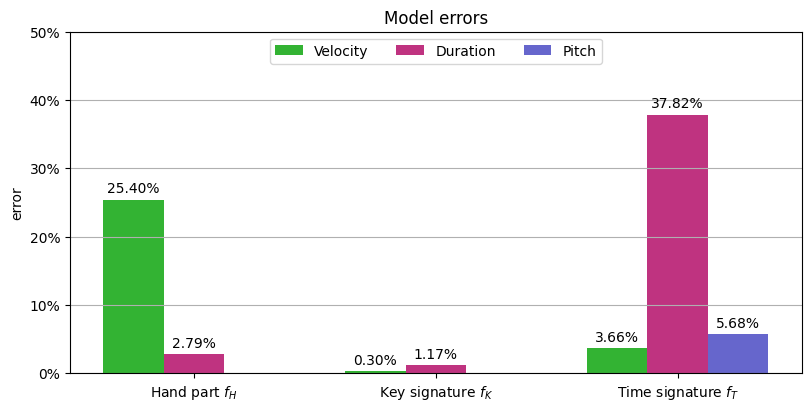
\includegraphics[width=0.96\textwidth]{images/ceteris_paribus_results.png}
\caption[\emph{Ceteris paribus} analysis model errors]{\emph{Ceteris paribus} analysis model errors.}
\label{ceteris_paribus}
\end{figure}

\subsection{Local Feature Importance}

We encountered challenges with common explainable machine learning tools: 

\begin{itemize}[noitemsep, topsep=4pt]
	\item Input data is a tensor of variable length, not conforming to tabular or image-like formats supported by many tools.
	\item The input data is a very high-dimensional space, computationally infeasible for certain methods (e.g. Shapley values).
	\item Pitch perturbations introduce non-integer values, and the pitch space lacks a meaningful measure of distance.
	\item Some model components (e.g. GRU blocks, ELU activation function) are not supported by certain XAI libraries.
\end{itemize} 

We developed a custom solution to overcome these obstacles. For velocity, we applied a LIME-like approach due to the absence of metric structure in the pitch space. We generated a locally modified version of the MIDI stream tensor for each note, randomizing the velocity for one note. We created $100$ samples for each note, calculating model predictions to compare with the original prediction. This approach aids in explaining the findings from the previous section (see Figure \ref{hand_part_misalignment} for an example).

We also measured the mean influence through this approach: the square root of the mean of squares of linear regression coefficients. This approach aligns with the \emph{ceteris paribus} analysis.

\begin{table}[ht!]
\[\begin{array}{c|ccc}
      \text{model}             & f_H           & f_K  & f_T  \\\hline
      \text{average influence} & \textbf{0.37} & 0.04 & 0.05
\end{array}\]
\caption{The average influence of three models calculated by a LIME-like approach.}
\end{table} 

However, the proposed approach ignores the feature interaction and silently assumes variable independence, both horizontally and vertically. This is a serious limitation of this approach. 

\subsection{Key Signature Assignment by Note Omission}

For the key signature model, as the pitch space is not a metric space, we applied a different strategy. The method is as follows: 
\begin{enumerate}[noitemsep, topsep=4pt]
	\item Get the key signature prediction values (before the last activation function) for the entire sequence.
	\item Individually remove each note in a sequence and calculate the difference between the original prediction and the prediction made on a sequence without a single note.
	\item Compute a contribution score, represented by the mean of the differences for each note.
	\end{enumerate} This approach enables the measurement of each note's contribution to the attribution of a specific scale. Refer to Figure \ref{note_removing} for an illustrative example.

\subsection{Conclusion}

We were able to discover certain artifacts of the score generation models, especially when it comes to velocity contribution to hand part assignment. The time signature model is not fully robust to alterations that should not have affect the output.

Unfortunately, the proposed methods have drawbacks and are not fully justified. Current XAI methods do not work well with symbolic music data in general. Developing more tailored and adaptable XAI methods for musical applications could contribute to improved model interpretability. One of the challenge would be to find a reasonable (and interpretable) embedding of the pitch space that encodes musical features. 

\begin{figure}[!ht]
\centering
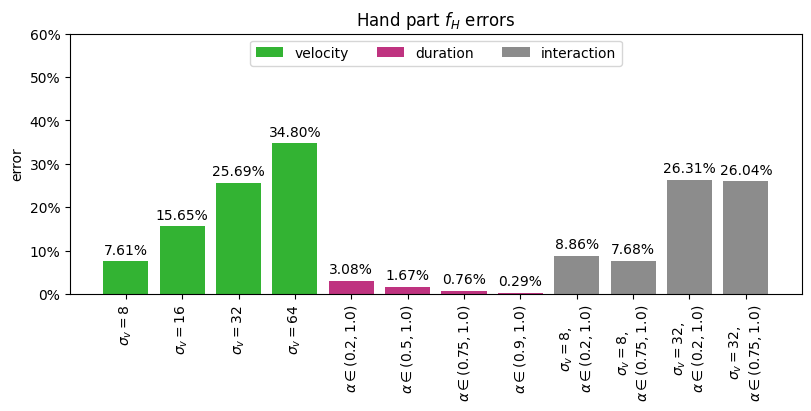
\includegraphics[width=0.7\textwidth]{images/ceteris_paribus_results_h.png}
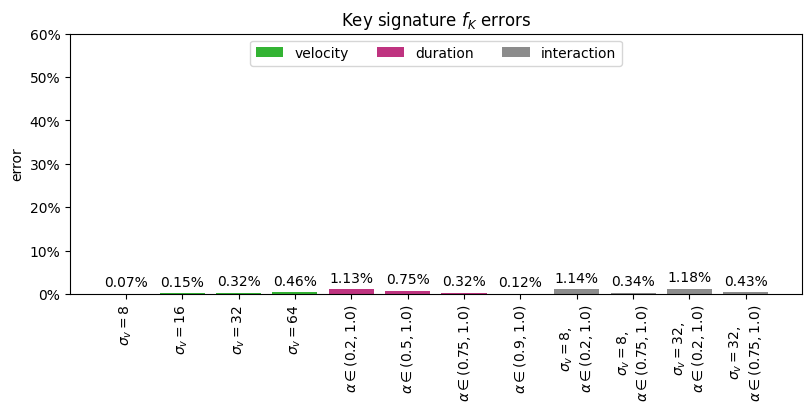
\includegraphics[width=0.7\textwidth]{images/ceteris_paribus_results_k.png}
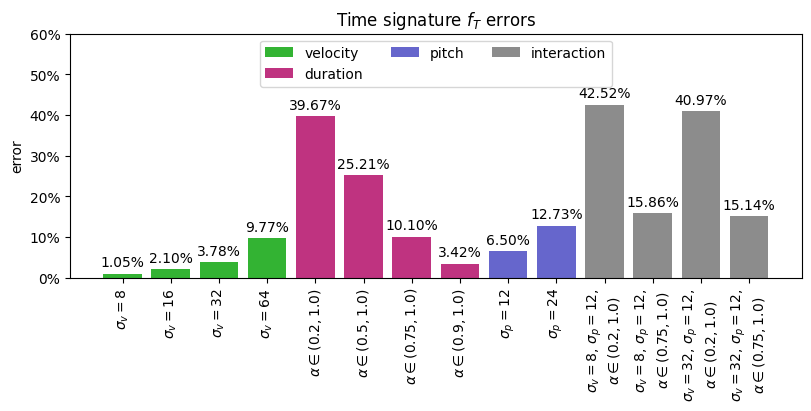
\includegraphics[width=0.7\textwidth]{images/ceteris_paribus_results_t.png}
\caption[Results of the \emph{ceteris paribus} experiment]{Results of the \emph{ceteris paribus} experiment for the hand part model $f_H$, the key signature model $f_K$ and the time signature model $f_T$. The hand part model is robust to note duration changes while it is susceptible to velocity manipulation. On the other hand, the time signature model is sensitive to note duration changes, which is expected to some extent, and relatively robust to other transformations. The key signature model is robust to all perturbations.}
\label{ceteris_paribus}
\end{figure}

\begin{figure}[!ht]
\centering
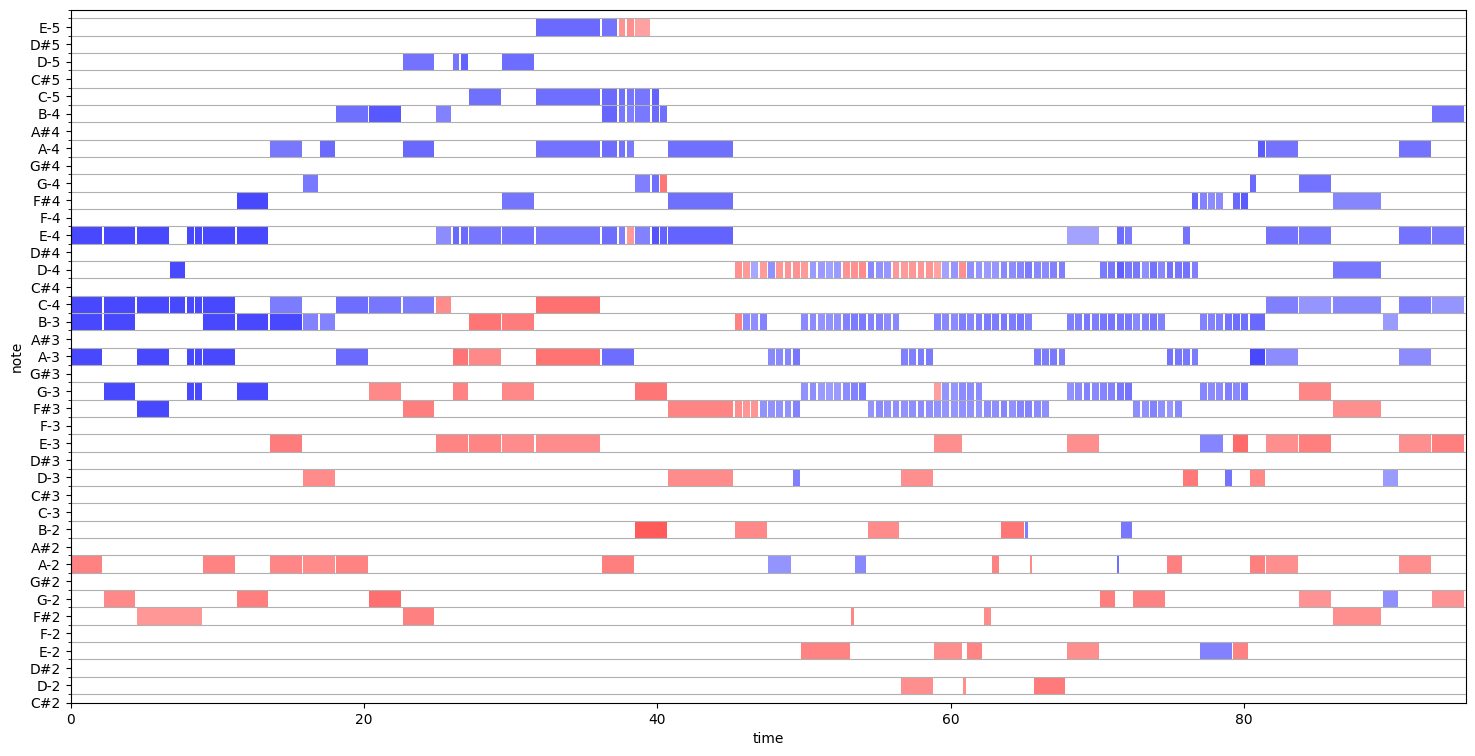
\includegraphics[width=0.95\textwidth]{images/hand_part1.png}
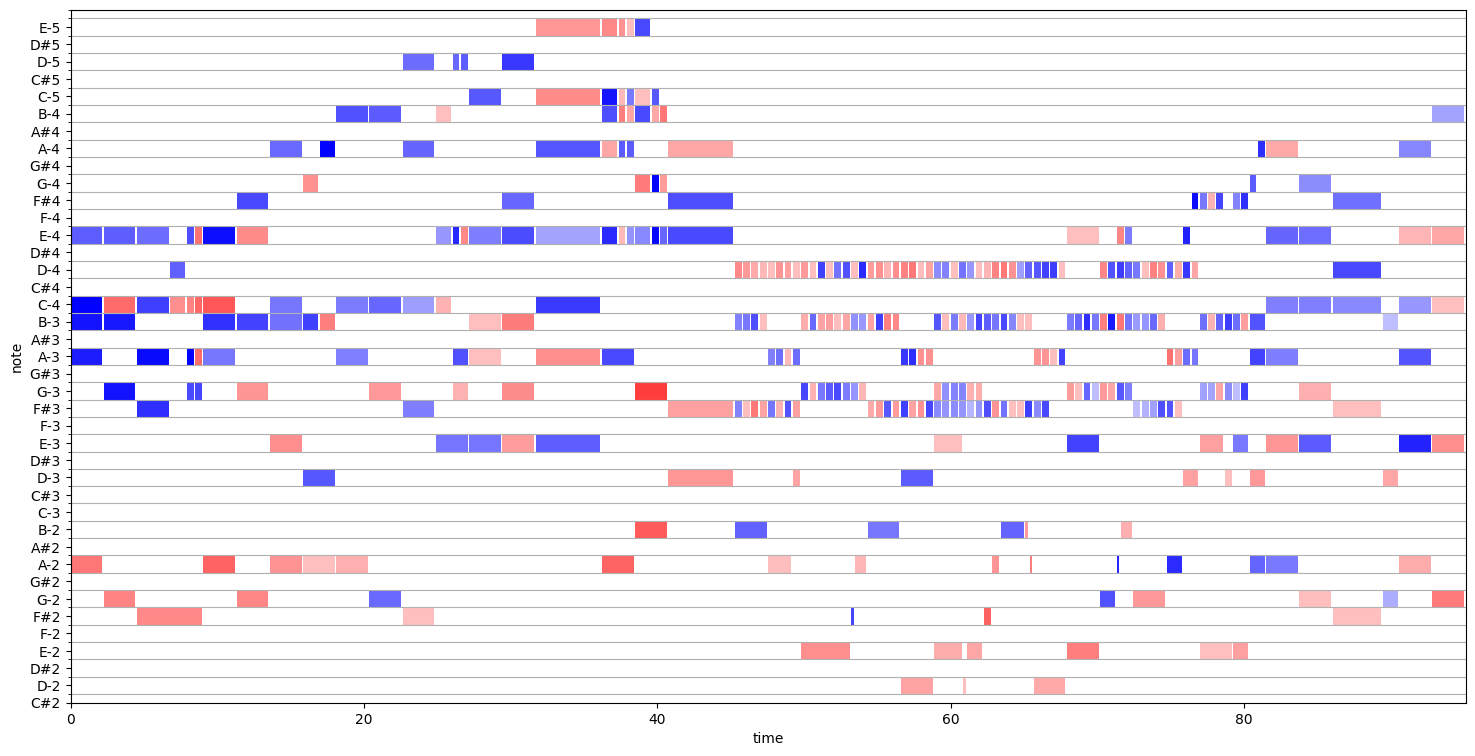
\includegraphics[width=0.95\textwidth]{images/hand_part2.png}
\caption[The piano roll for the hand part model output]{The piano roll for the hand part model output. Each note is represented as a (blue or red) block, indicating a pitch (note), duration and velocity. The first graph represents an original sequence while the second has perturbed velocity. Left-hand notes are marked as red. We can see that there are much many misalignment in the hand assignment in the second output. As a rule of thumb, the left hand notes (red) should be at the bottom while the right hand ones (blue) should be at the top.}\end{figure}

\begin{figure}[!ht]
\centering
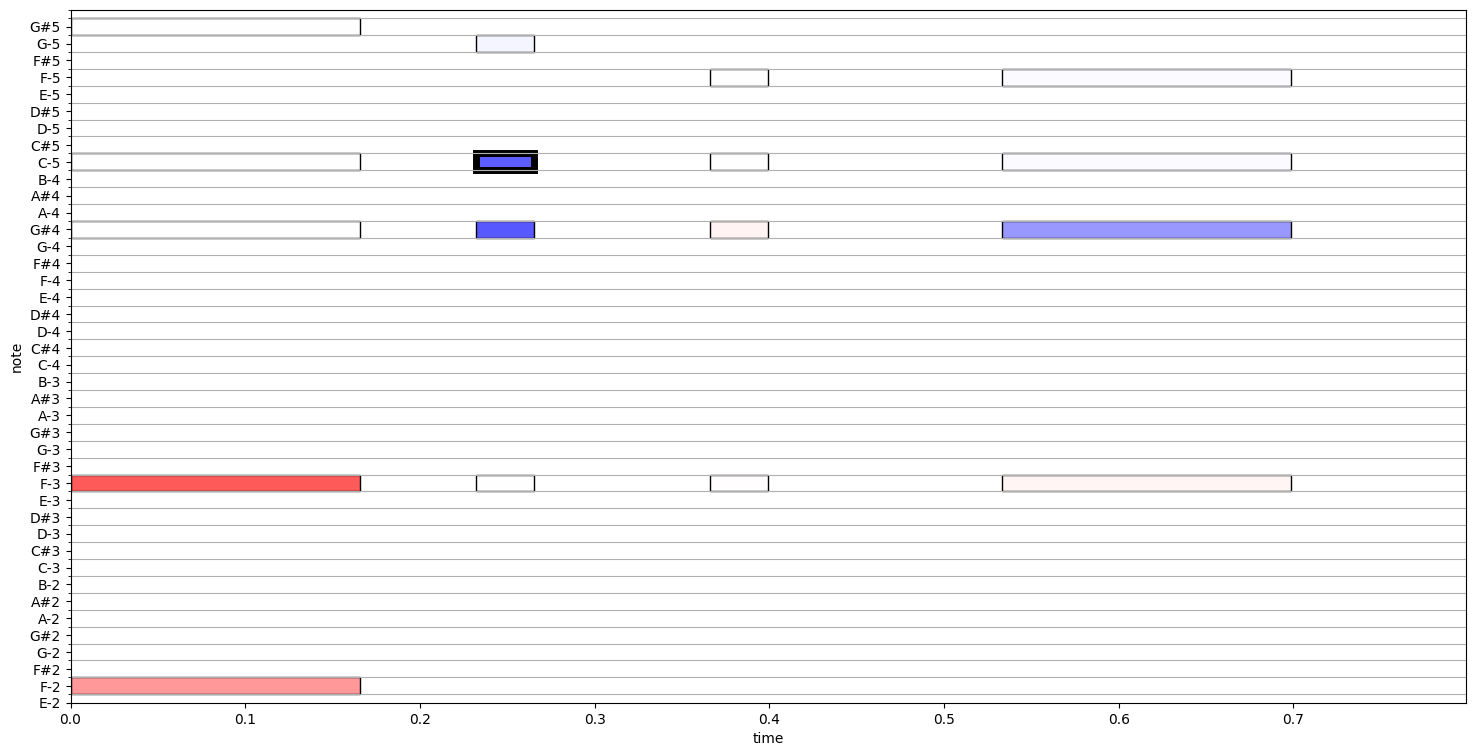
\includegraphics[width=0.95\textwidth]{images/lime_hand_part.png}
\caption[A graph showing how the velocity of a note influences hand part assignments of other notes]{A graph showing how the velocity of the second C5 note (with a thick outline) influences hand part assignments of other notes. It can be observed that the current velocity of this note makes the model think of the first F3 note as a left hand note. Reducing the note C5 velocity to a low value results in a misassigning F3 as the right hand note. This is, of course, a undesired behavior of the model.}
\label{hand_part_misalignment}\end{figure}

\begin{figure}[!ht]
\centering
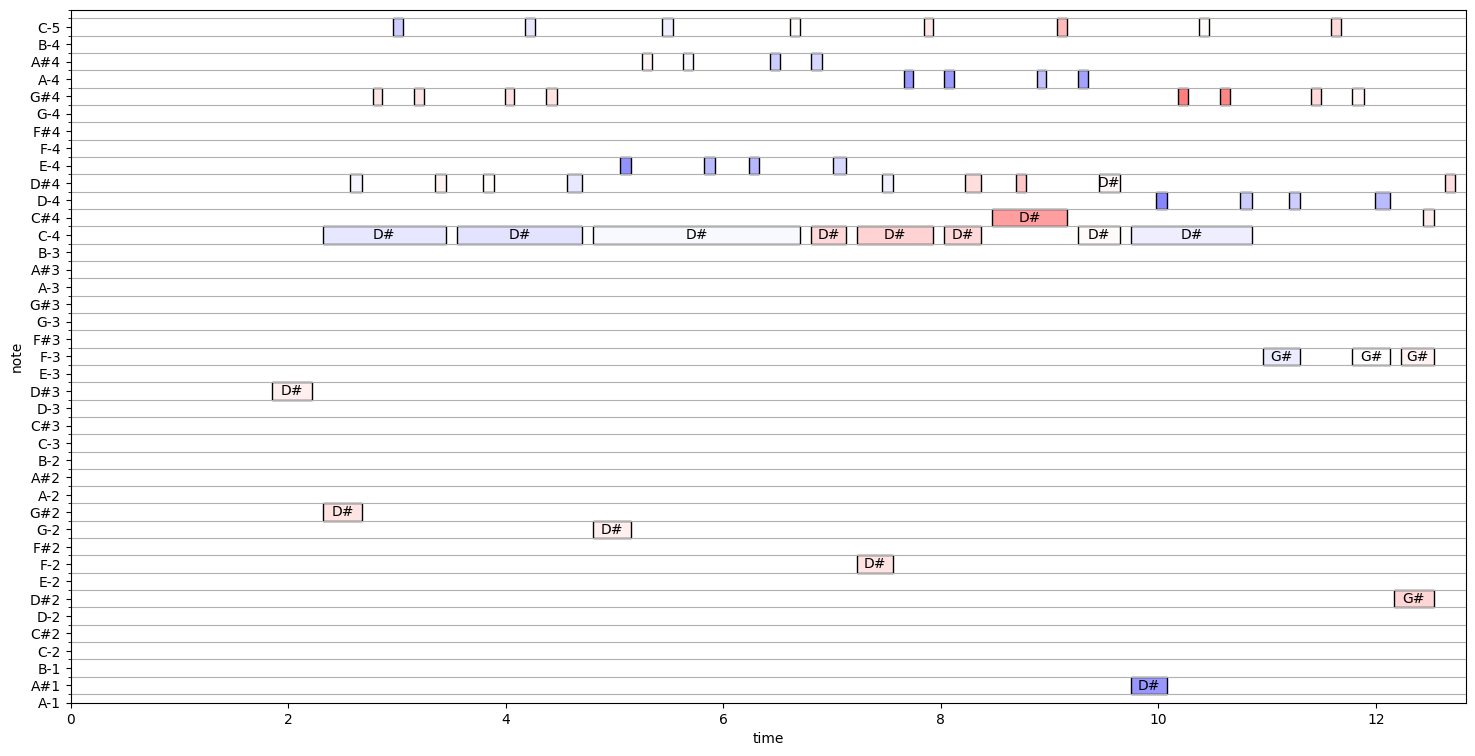
\includegraphics[width=0.95\textwidth]{images/note_removing.png}
\caption[A key signature alignment for D$\sharp$ scale]{A key signature alignment for D$\sharp$ scale. The names on the notes represent the model key signature attribution. There are two different scales assigned by the model: D$\sharp$ scale and G$\sharp$ scale. Notes: D, E and A are not in the scale and have a negative influence on the assignment.}
\label{note_removing}\end{figure}
